\documentclass{labReport}
\urlstyle{same}

\let\verbatim\undefined 
\let\verbatimend\undefined 
\lstnewenvironment{verbatim}{\lstset{breaklines,basicstyle=\ttfamily}}{}
\usepackage{lipsum}

\title{Lab 4: Divide and Conquer Algorithms}
\author{Adam Haile, Aiden Miller, Leigh Goetsch}
\prof{Dr. Berisha}
\className{Algorithms \& Adv. Data Struct.}
\classCode{CSC 3310}
\semester{Fall 2024}
\submissionDate{11/08/2024}
\labWeek{8}
\laboratoryDate{10/25/2024}

\begin{document}
\maketitle

\section*{Learning Outcomes}
\begin{itemize}
    \item Design an algorithm for a given computational problem statement
    \item Justify the correctness of an algorithm
    \item Perform asymptotic complexity analysis of the run time of an algorithm
    \item Generate test cases for an algorithm
    \item Correctly implement an algorithm from pseudocode
    \item Design and execute benchmarks for an algorithm
\end{itemize}

% if you want a TOC:
% \tableofcontents

\newpage
% if you want to use multicols:
\begin{multicols*}{2}
\raggedcolumns



\section{Approach}
% A paragraph describing the approach that you used to solve the problem. Provide at least 2 illustrations that explain the approach
The quickselect algorithm utilizes divide-and-conquer to find the $k^{th}$ smallest element without sourting the entire array. The key idea is to repeatedly partition the array using a randomly chosen pivot. During each partition, elements smaller than the pivot get moved to the left and greater elements are moved to the right. If the pivot's index is exactly $k - 1$, we have found the $k^th$ smallest element. Otherwise, we will continue searching recursively in the relevant subarray, reducing the problem size at each step. 
\begin{figure}
     \centering
     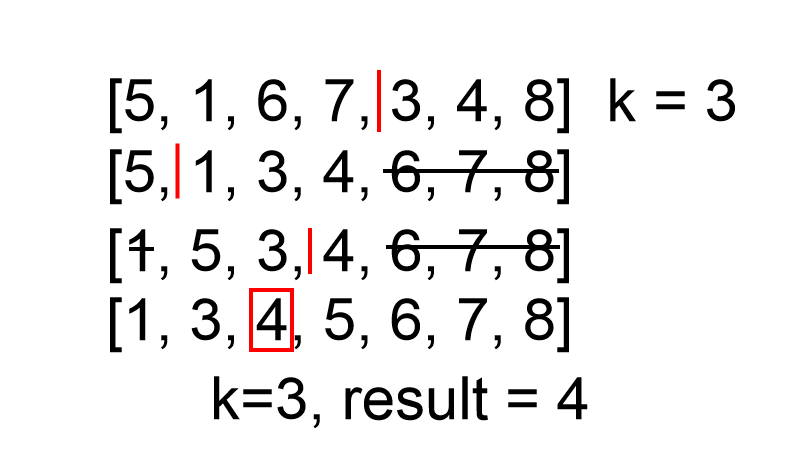
\includegraphics[width=1\linewidth]{Quickselect.png}
\end{figure} 



\section{Pseudocode}
% High-level pseudocode for an algorithm that uses that rule to solve the computational problem for any input
\begin{verbatim}
partition(lst, low, high):
    SWAP(lst[RANDOM(low, high)], lst[high])
    pivot = lst[high], i = low
    FOR j FROM low TO high - 1:
        IF lst[j] < pivot: SWAP(lst[i], lst[j]), i = i + 1
    SWAP(lst[i], lst[high])
    RETURN i

select(lst, low, high, k):
    IF low = high: RETURN lst[low]
    pivot_index = partition(lst, low, high)
    IF k = pivot_index: RETURN lst[k]
    RETURN select(lst, low, pivot_index - 1, k) IF k < pivot_index ELSE select(lst, pivot_index + 1, high, k)

quickselect(lst, k):
    RETURN select(lst, 0, LENGTH(lst) - 1, k - 1)
\end{verbatim}

\section{Algorithm Justification}
% 3. Provide an explanation and justification for why your algorithm is correct (1-3 paragraphs)
The quickselect algorithm is able to solve the k-smallest problem using divide-and-conquer similar to how Quicksort operates. It is able to narrow the search space by partitioning the array around a randomly chosen pivot element. Each partition step ensures the pivot element is in a correct sorted position, with all smallest elements to the left and larger elements to the right. If the pivot's position is equal to $k - 1$, it is the $k^{th}$ smallest element. Otherwise, it will recursively ssearc the subarray to the left or right depending on the position of k comparatively to the array sizes.


\section{Test Cases}
% A table of your test cases, the answers you expect, and the answers returned by running your implementation of the algorithm
\begin{table}[h!]
    \centering
    \begin{tabular}{|c|c|}
    \hline
    Test & Description & Result \\
    \hline
    Test 1 & Test 10 elements to ensure that the kth smallest element corresponds to the [k-1]th index of a sorted list & Pass \\
    Test 2 & Test to ensure that lots of duplicate elements are handled correctly & Pass \\
    Test 3 & Test wildly small and large values & Pass \\
    Test 4 & Shuffle list and test, ensuring that there isn't a dependence on ordering & Pass \\
    Test 5 & 2 element list & Pass \\
    Test 6 & 10000 element list & Pass \\
    \hline
    \end{tabular}
    \caption{Test Results}
    \label{table:test_results}
\end{table}

\section{Recurrence Relation}
% Derive a recurrence relation describing the run time in terms of the number of points n. (Hint: assume that the random pivot divides the elements in half each time.
% Solve the recurrence relation to get a run time in terms of n in asymptotic notation
The recurrence relation is:
$T(n) = T(\frac{n}{2})+O(n)$
Using the master theorem, we get that this is a Case 3 recurrence relation, which tells us that the average case time complexity of this algorithm is $T(n) = O(n)$

\section{Benchmarking}
% Benchmark your implementation versus an approach that sorts the numbers and picks the element at index k – 1. You should include a table and graph from benchmarking different lists with different sizes of numbers. The benchmarks should support your theoretically-derived run time and provide evidence that the run time of your algorithm grows more slowly than the sorting approach.

\end{multicols*}

% add appendix
% 7. Attach all your source code and test cases in an appendix.



\end{document}
